\chap{Discussion}
Is possible to say that the obtaiend results are achieving most of the initil goals of this project. 
Like reported in the introduction part [\ref{Introduction}], the two main goals of this work were: 
\vspace{-5mm}
\begin{itemize}
 \setlength{\itemsep}{-5pt}
 \item Implement a web application that provides a scheduler.
 \item Apply the development agile process.s
\end{itemize}

The resulting web application actually provides a online scheduler that contains several utilities and functions. Almost all the user stories that were supposed to be realized have been correctly implemented. In particular, the results provide an answer to the initial goals of the scheduler implementation. 

Further more, during the whole development process the agile approach had a high consideration and priorization from all the members of the team. Has been actually possible to see a big improvement about the agile process application between the beginning and the end of this work.

More details about evaluation and limitations of the implemented project can be find in the next section.
\section{Evaluation and Limitations}
\vspace{-5mm}
\label{Evaluation}
The following list reports the main limitations that have been encountered during the implementation process.
\vspace{-5mm}
\begin{itemize}
 \setlength{\itemsep}{-5pt}
\item Time limitation has probably been the biggest issue. Working on a project with several people means that you have to somehow find a way to combine different schedules, that is not always that easy. Also a quite short project deadline implies a limitated extra features implementation.
\item Limitated amount of previous knowledges and experiences about both Ruby on Rails and agile process imply that each single member of the team, mainly during the first part of the work, had to document himself about it. It means a significant investment of time and effort focused about get knowledge and less about web application's extra features. 
\end{itemize}

Despite of the limitations that have been reported above here, this work provided to all the team member:
\vspace{-5mm}
\begin{itemize}
 \setlength{\itemsep}{-5pt}
\item New knowledges and experiences about agile process, in particular how to handle a group project, communication and collaboration with other people.
\item Improved abilities about gitlab/github usage, since it has been an indispensable instrument during the whole work.
\item Fist but really complete approach with framework Ruby on Rails.
\end{itemize}



\section{Team efforts and Time lists}
\vspace{-5mm}
One of the most important thing during the whole development process was splitting the jobs between the team members in a efficient way and at the same time let every single team member put the same effort into the project.\\
Was actually asked to every single team member to constantly contribute at the work as much as possible. How it's possible to see in the following graphic, there has been a quite constant effort and work on the project.
\begin{figure}[H]
	\centering
    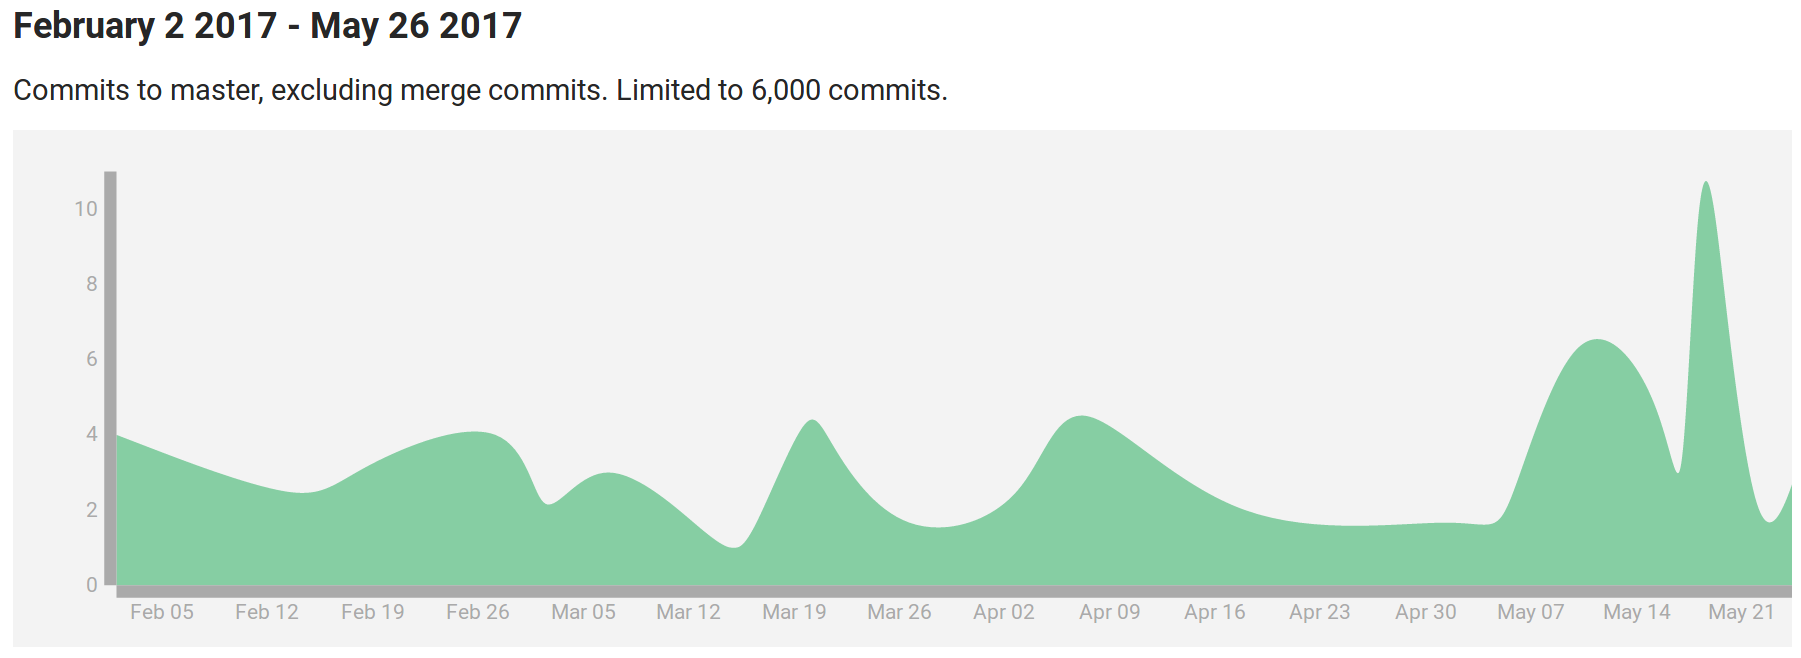
\includegraphics[trim={0 0 0 0},clip,width=1\textwidth]{Files/commitsToMaster.png}
    \caption{Commits to master, excluding merge commits.\\ \textbf{Source:} https://inf2900v17.cs.uit.no/team1/coffee-overflow/graphs/master}
    \label{fig: MVC}
\end{figure}


